\section{Overview: Results of Dataset}
\section{Discussion}
\subsection{Comparision to Experiment}

\begin{figure}
	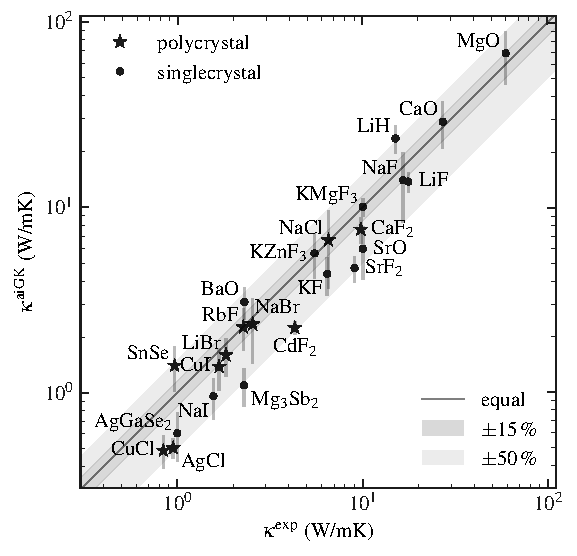
\includegraphics[width=\textwidth]{./data/plots/kappa_vs_exp_trusted/kappa_vs_exp_corrected_annotated.pdf}
	\caption{Comparison to experiment. Bullets($\bullet$): Single crystal. Stars ($\star$): Contains data from polycrystalline experiment. Error bar in y-direction: Statistical uncertainty for $\kappa^{\rm aiGK}$ from standard error over individual trajectories. Diagonal line: Agreement with experiment or mean of experiments if multiple available. Dark grey region: Agreement between mean experiment and mean computation with $\pm 15\,\%$ deviation. Light grey region: Agreement between mean experiment and mean computation with $\pm 50\,\%$ deviation.}
	\label{fig:kappa_exp}
\end{figure}



\subsection{Relation to Anharmonicity}

\begin{figure}
	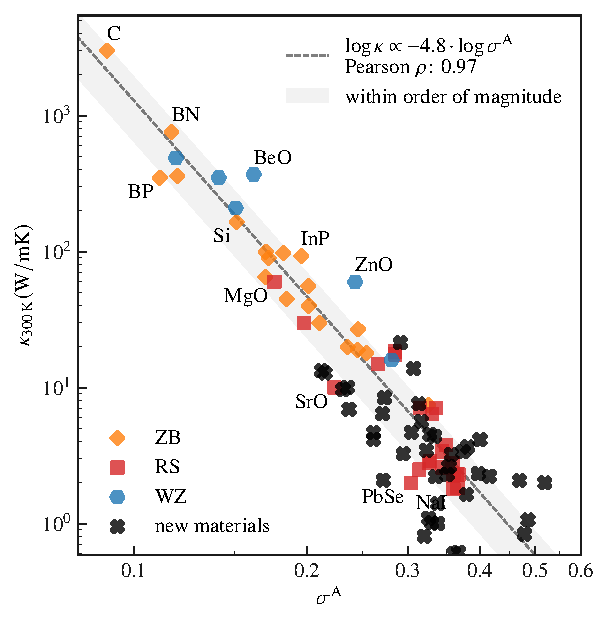
\includegraphics[width=\textwidth]{./data/plots/anharmonicity/9_kappa/incl_computations/sigma_vs_kappa_annot_comp.pdf}
	\caption{Thermal conductivity at room temperature vs. anharmonicity measure.}
	\label{fig:kappa_sigma_exp_comp}
\end{figure}

\begin{figure}
	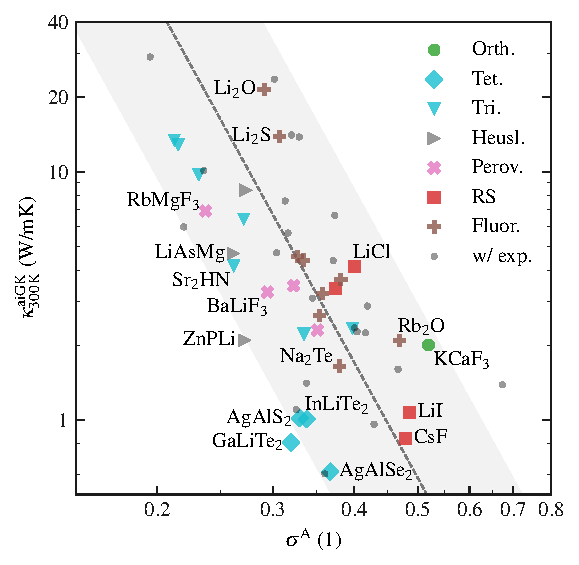
\includegraphics[width=\textwidth]{./data/plots/kappa_vs_sigma_trusted/kappa_vs_sigma_trusted.pdf}
	\caption{Thermal conductivity at room temperature vs. anharmonicity measure. Small grey dots denote materials where experimental reference was available. Other symbols denote materials where not experimental references where available before.}
	\label{fig:kappa_sigma}
\end{figure}

\newpage

\subsection{Chalcopyrites}
\begin{figure}
	\centering
	GaLiTe$_2$ \hspace{3.7cm} InLiTe$_2$\\
	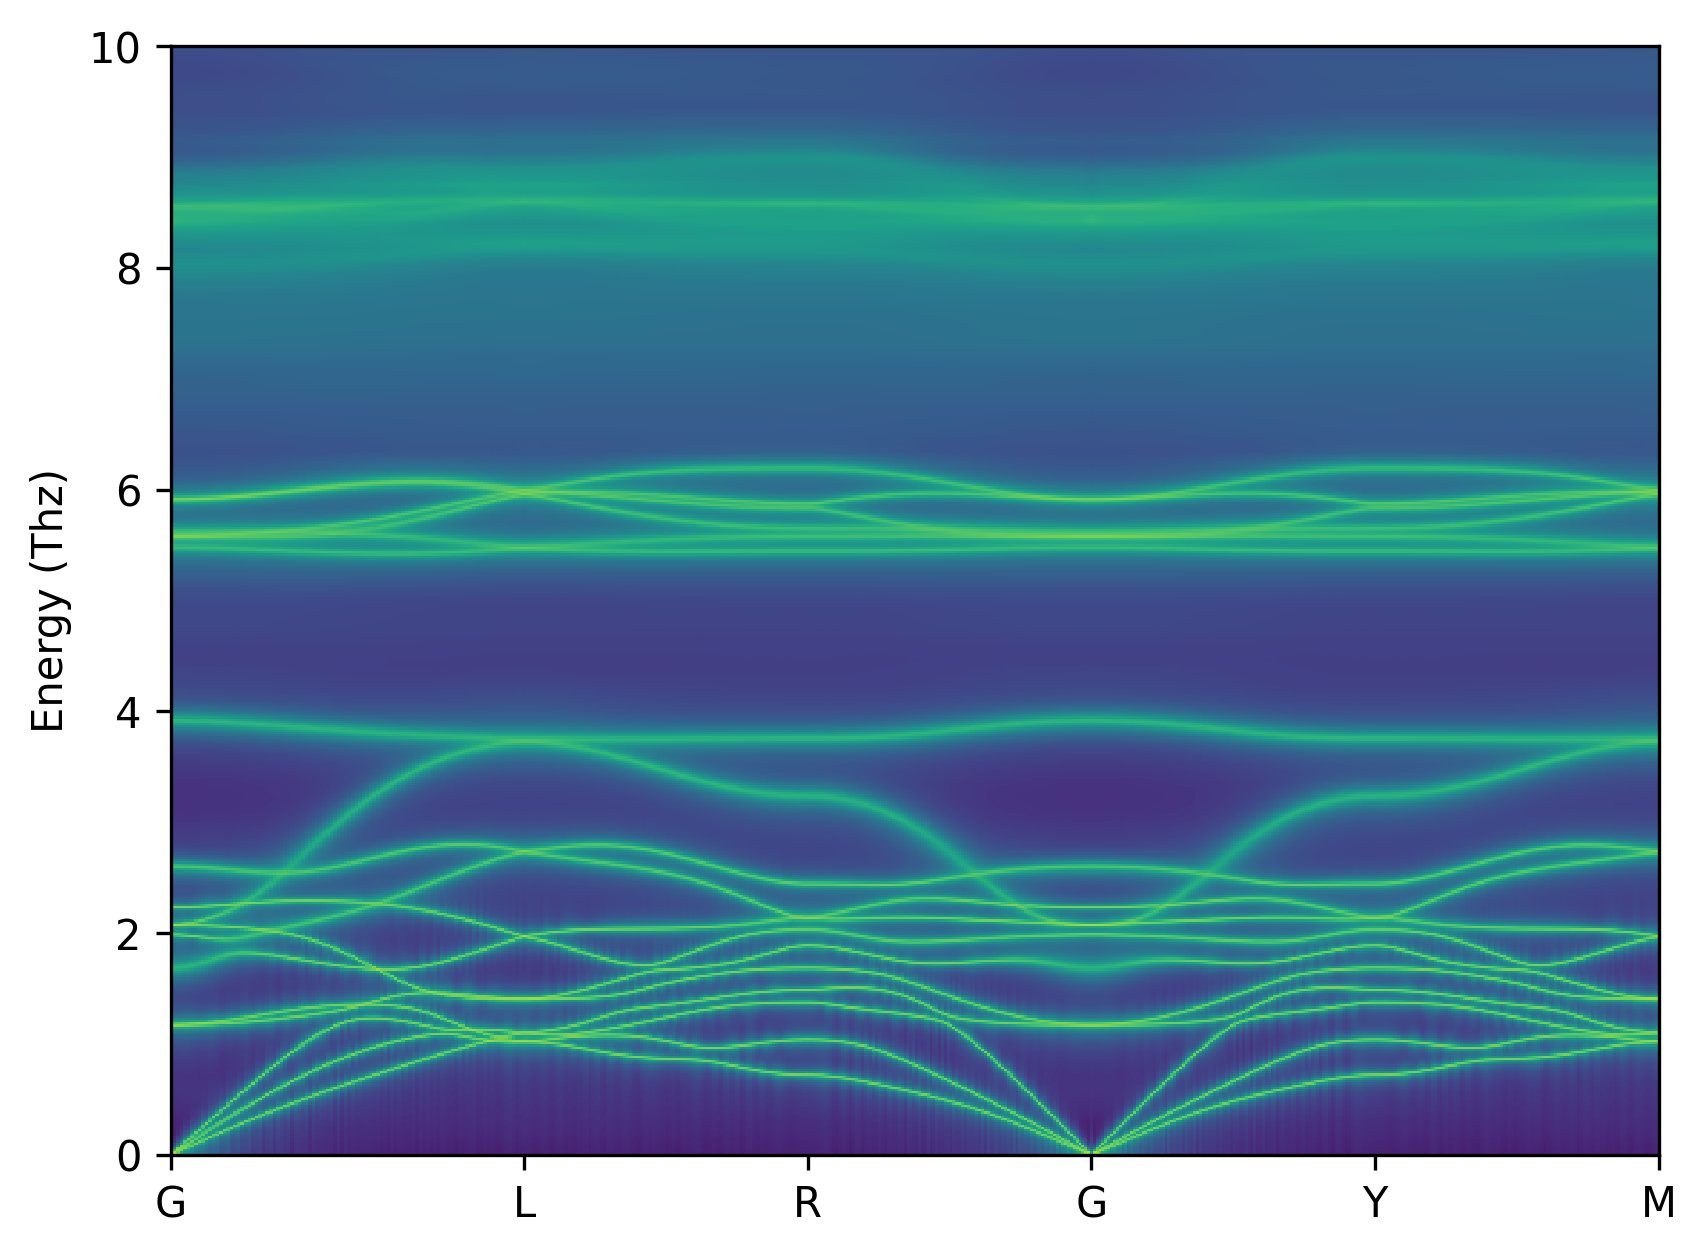
\includegraphics[width=0.45\textwidth]{./data/plots/spectral_functions/122.04.GaLiTe2.png}
	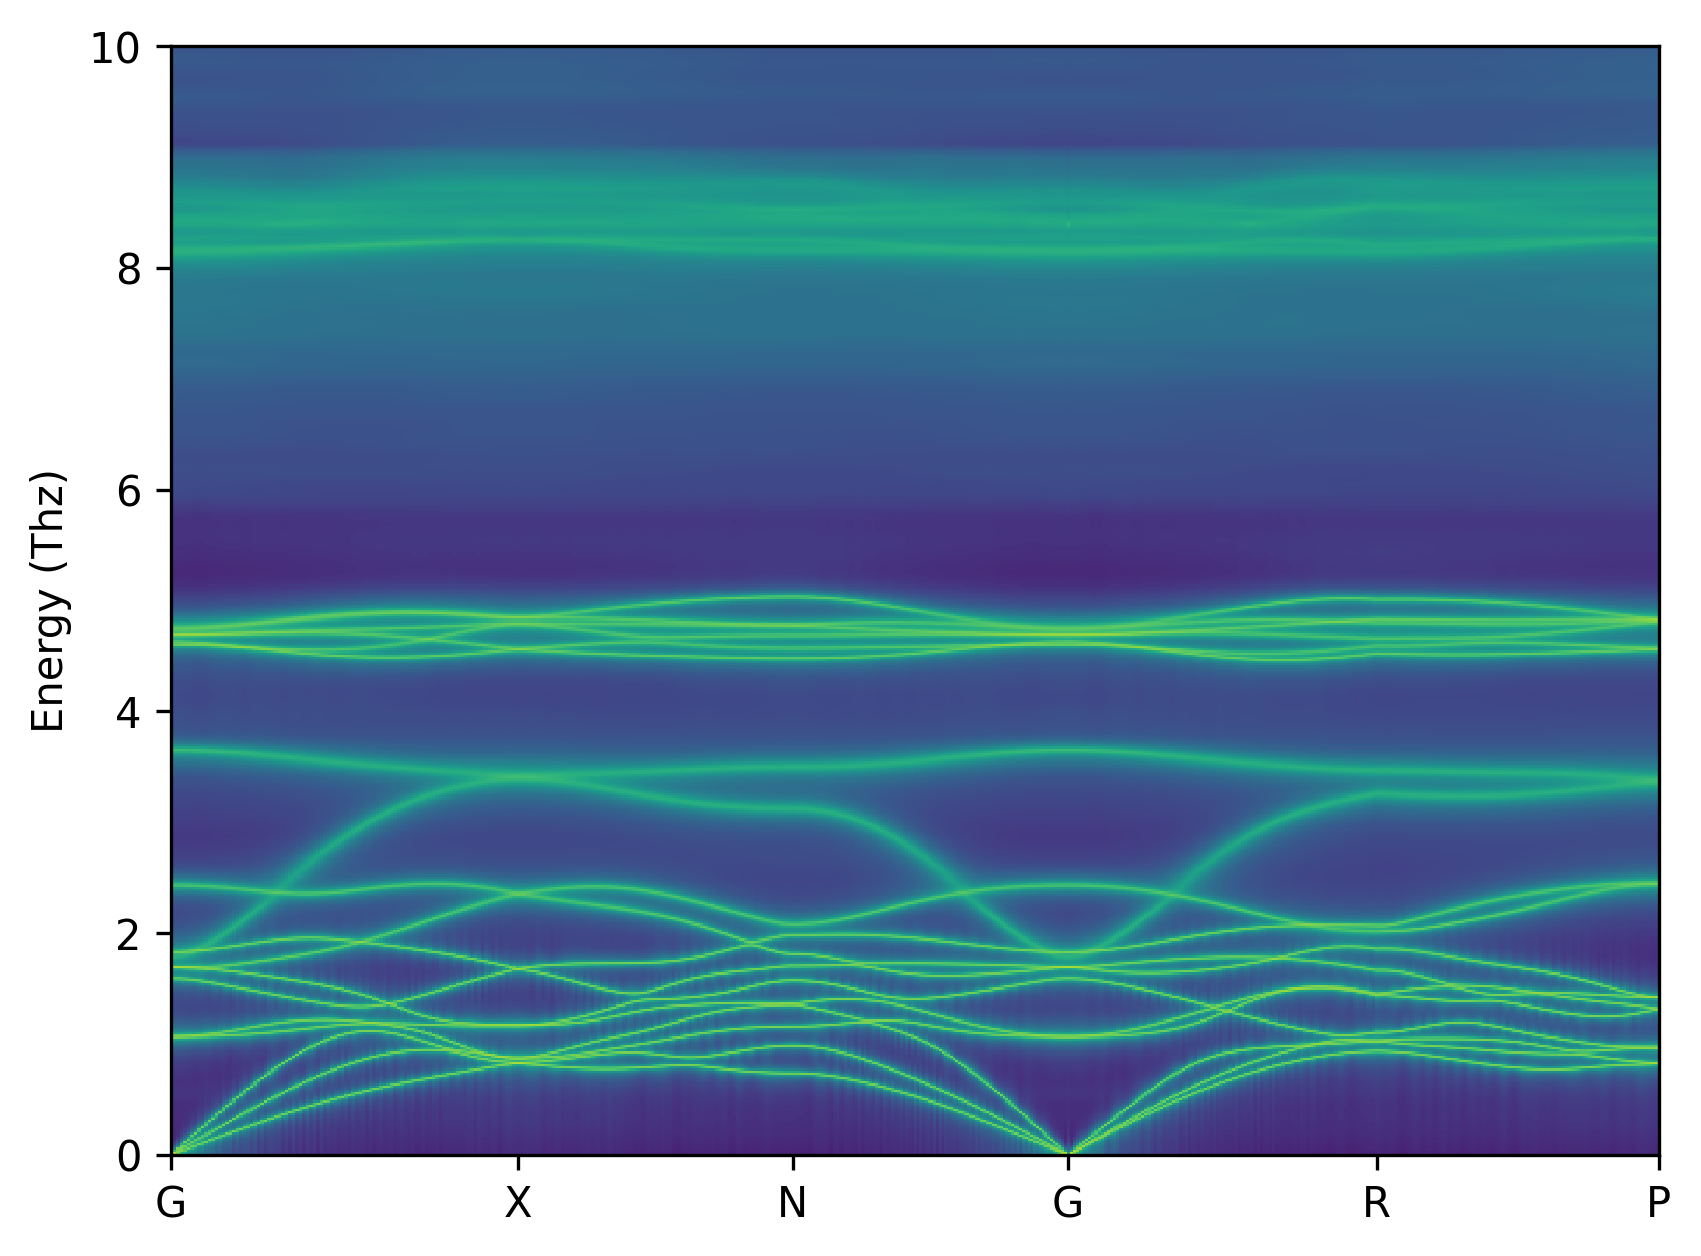
\includegraphics[width=0.45\textwidth]{./data/plots/spectral_functions/122.04.InLiTe2.png}
	\caption{Spectral functions for the chalcopyrite materials GaLiTe$_2$ and InLiTe$_2$.}
	\label{fig:kappa_sigma}
\end{figure}

\cite{kuhn1985,kuhn1987,isaenko2005}

\begin{table}[ht]
  \centering
  \fontfamily{ppl}\selectfont
\begin{tabular}{lrrr}
\toprule
     material &  kappa\_corrected &      sigma &  space\_group \\
\midrule
 InLiTe$_2$ &             0.46 &       0.33 &          122 \\
 GaLiTe$_2$ &             0.47 &       0.31 &          122 \\
  AgAlS$_2$ &             0.84 &       0.33 &          122 \\
        CsF &             0.84 &       0.48 &          225 \\
        LiI &             1.07 &       0.49 &          225 \\
   Na$_2$Te &             1.64 &       0.38 &          225 \\
   KCdF$_3$ &             1.67 &       1.32 &           62 \\
   KCaF$_3$ &             2.00 &       0.52 &           62 \\
    Rb$_2$O &             2.08 &       0.47 &          225 \\
      ZnPLi &             2.09 &       0.27 &          216 \\
 InNaSe$_2$ &             2.22 &       0.34 &          166 \\
  CsCdF$_3$ &             2.30 &       0.35 &          221 \\
 InLiSe$_2$ &             2.34 &       0.40 &          166 \\
   Na$_2$Se &             2.63 &       0.35 &          225 \\
   Li$_2$Te &             3.24 &       0.36 &          225 \\
  BaLiF$_3$ &             3.27 &       0.29 &          221 \\
         KH &             3.39 &       0.37 &          225 \\
  RbZnF$_3$ &             3.47 &       0.32 &          221 \\
     K$_2$O &             3.67 &       0.38 &          225 \\
       LiCl &             4.14 &       0.40 &          225 \\
   Sr$_2$HN &             4.17 &       0.26 &          166 \\
    Na$_2$S &             4.40 &       0.33 &          225 \\
   Li$_2$Se &             4.55 &       0.33 &          225 \\
     LiAsMg &             4.67 &       0.26 &          216 \\
  LiScS$_2$ &             6.42 &       0.27 &          166 \\
  RbMgF$_3$ &             6.94 &       0.24 &          221 \\
      LiNZn &             8.42 &       0.27 &          216 \\
  InNaO$_2$ &             9.71 &       0.23 &          166 \\
  CuGaO$_2$ &            12.82 &       0.22 &          166 \\
  LiRhO$_2$ &            13.37 &       0.21 &          166 \\
    Li$_2$S &            13.85 &       0.31 &          225 \\
    Li$_2$O &            21.39 &       0.29 &          225 \\
\bottomrule
\end{tabular}
  \caption{Thermal conductivities without experimental reference.}
  \label{tab:kappa.noexp}
\end{table}